\section{Comparison with experimental data}
Numerical experimental data from the provided reference could only be obtained for angles of
attack of 0 and 10 degrees, thus the comparison will be performed for these
angles instead. Moreover, said data is only available for the upper surface.

\Cref{fig:q2} compares the inviscid and viscous results, using PABLO, against
the experimental data.

\begin{figure}
    \centering
    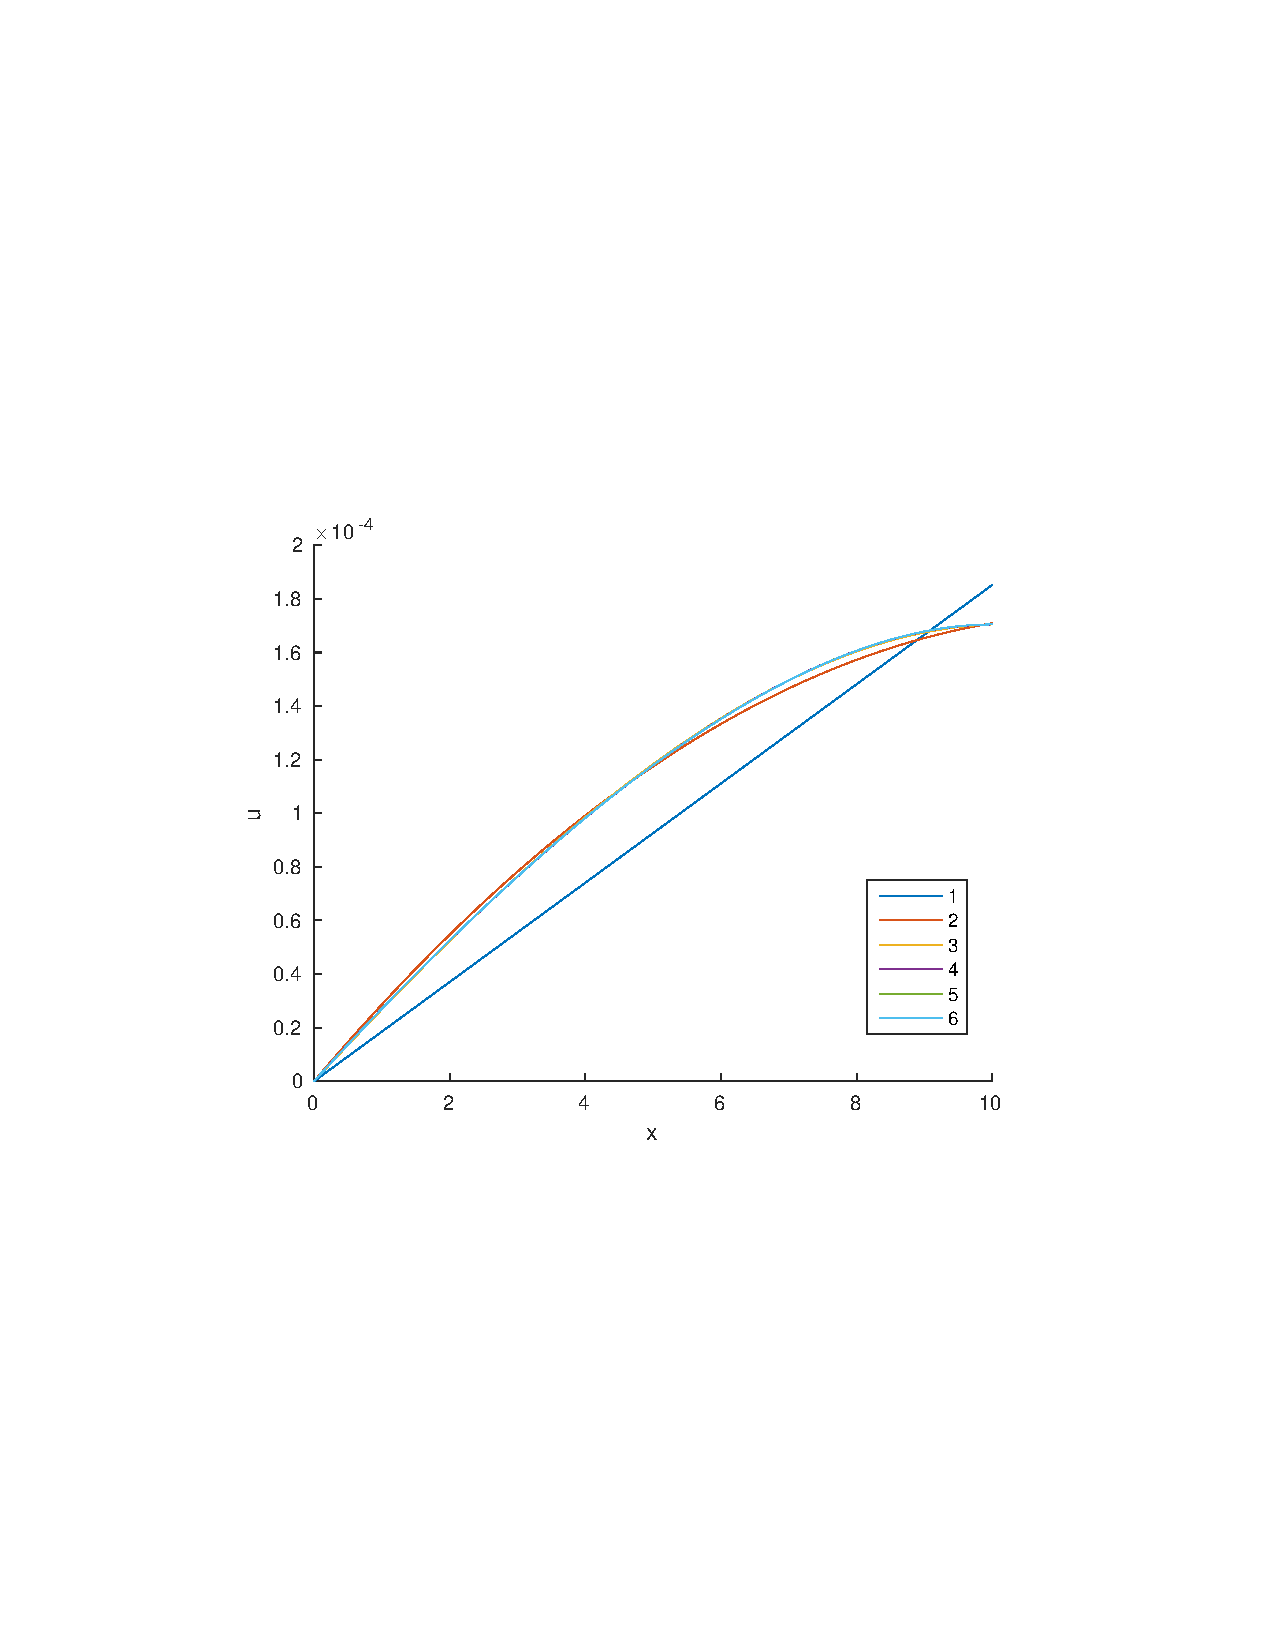
\includegraphics[width=1.0\textwidth]{./figs/q2}
    \caption{Comparison of NASA's experimental data with PABLO's viscous
        and inviscid results. The latter two results are identical.}\label{fig:q2}
\end{figure}

\subsection{Effect of viscosity}
The first thing to notice is that PABLO's viscous and inviscid solutions are exactly
the same. As a matter of fact, toggling the ``Viscous'' has absolutely no effect on
the computed pressure distribution. The boundary layer (BL) solver and potential flow (PF)
solver are completely decoupled and the overall solve is not iterative, meaning both
solvers are only run once. Specifically, the velocity field is output from the PF solver
and input into the BL solver.

\subsection{Comparison}
From~\Cref{fig:q2}, it can be said that the experimental and PABLO results are relatively close.
However, there are slight discrepancies specifically at the airfoil's trailing edge: the pressure
from PABLO increases significantly right at that location, unlike the experimental results. In
other words, the fluid undergoes a large deceleration.
